\documentclass[draftclsnofoot, onecolumn, compsoc, 10pt]{IEEEtran}
\usepackage{lscape}
\usepackage{rotating}
\usepackage{titling}
\usepackage[margin=0.75in]{geometry}
\usepackage{graphicx}
\usepackage{placeins}
\usepackage{caption}
\usepackage{float}
\usepackage{url}
\usepackage{listings}
\usepackage{natbib}
\usepackage{setspace}
\geometry{textheight=9.5in, textwidth=7in}
\graphicspath{ {images/} }
\linespread{1.0}
\parindent=0.0in
\parskip=0.2in

\title{OS 2 Assignment 4}
\author{Oregon State University\\CS 444\\2018\\\\Prepared By:\\Hayden
Anderson\\Thomas Noelcke\\James Zeng\\}


\def \CapstoneTeamNumber{		41	}
\def \CapstoneProjectName{		Assignment 4 }




\newcommand{\NameSigPair}[1]{\par
\makebox[2.75in][r]{#1} \hfil 	\makebox[3.25in]{\makebox[2.25in]{\hrulefill} \hfill		\makebox[.75in]{\hrulefill}}
\par\vspace{-12pt} \textit{\tiny\noindent
\makebox[2.75in]{} \hfil		\makebox[3.25in]{\makebox[2.25in][r]{Signature} \hfill	\makebox[.75in][r]{Date}}}}

\begin{document}
\begin{titlepage}
    \pagenumbering{gobble}
    \begin{singlespace}
        \hfill
        \par\vspace{.2in}
        \centering
        \scshape{
            \huge OS 2 \par
            {\large\today}\par
            \vspace{1in}
            \textbf{\Huge\CapstoneProjectName}\par
            \vspace{1in}
            {\large Prepared by }\par
            Group\CapstoneTeamNumber\par
            \vspace{5pt}
            \vspace{20pt}
        }
        \vfill
    \end{singlespace}
    \begin{abstract}
    \end{abstract}
\end{titlepage}
\newpage
\pagenumbering{arabic}
\clearpage
\tableofcontents
\pagebreak

\section{Solution Design}
    \subsection{Introduction}
    The following sections discuss the best fit and first fit algorithms in memory management and how we implemented them for this assignment. We also discuss how we plan on testing these algorithms.\\

    \subsection{First Fit}
    For the first fit algorithm, the memory allocates the first page available that is large enough for the payload to fit. The first first algorithm is already implemented and used in the SLOB slab. If no current page is large enough, it will create a new page that is big enough to accommodate the payload.\\

    \subsection{Best Fit}
    For the best fit algorithm we are going to group the memory needed by a small, medium, and large size. When a payload comes in, we check the size of the memory it needs and place the it into the corresponding page size needed for the slab.\\

    \subsection{Testing}
    To test these algorithms we will use a simple for loop that allocates memory of random sizes. It will create a large amount of allocations and then run our amount calculator. The amount calculator will use system calls to find the amount of memory allocated and divide that by the total amount of memory in use. This will give a percentage of performance for each algorithm.\\

\section{questions}
    \subsection{What Do you think the main point of this assignment is?}
    To understand the algorithms used in memory management and to get a hang of what algorithm is actually best to use for optimization, overhead, and less fragmentation.\\

    \subsection{How did you personally approach the problem? Design decisions, algorithm, etc.}
    We started off with some research to familiarize ourselves more on what the SLOB slab was and how it worked. We then researched a little on the how the first fit and best fit algorithm worked to give us better ideas on how we could implement it. After our research, we went through each of the files we needed to change to add the best-fit algorithm. Then we implemented our solution and tweaked it until it worked. Finally, we added a test script that would allocate random memory a bunch of times and added printk statements to see how effective the memory management was.\\

    \subsection{How did you ensure your solution was correct? Testing details, for instance. Ensure this is written in a way that the TA's can follow to ensure correctness.}
    We made tests with printk statements. We needed to find the percentage of actual used memory to the amount of memory being taken up when running. We knew we needed to allocate a bunch of memory of random sizes, then we needed to use system calls to get the actual amount of memory used and divide that by the total amount of memory taken up to find the effectiveness of the algorithm. We did this test for both algorithms and compared them by percentage.\\
  \begin{enumerate}
            \item First, we need to source the necessary configuration file.\\

\begin{lstlisting}
cp /scratch/opt/config-3.19.2-yocto-standard
source /scratch/opt/environment-setup-i586-poky-linux
\end{lstlisting}
            \item Change the name of the regular slob file to slob.c
\begin{lstlisting}
cd mm
mv slob_og.c slob.c
cd ..
\end{lstlisting}

            \item clean the kernel to ensure a sanitary environment.\\
\begin{lstlisting}
make clean
\end{lstlisting}
            \item make the kernel.
\begin{lstlisting}
make -j4 all
\end{lstlisting}
            \item run the kernel.
\begin{lstlisting}
qemu-system-i386 -redir tcp:5541::22 -nographic -kernel arch/x86/boot/bzImage -drive
file=core-image-lsb-sdk-qemux86.ext4 -enable-kvm -usb -localtime --no-reboot --append
"root=/dev/hda rw console=ttyS0 debug"
\end{lstlisting}
			\item Make the test script
\begin{lstlisting}
cd testfiles
make
\end{lstlisting}
			\item transfer the test files onto the VM
\begin{lstlisting}
scp -P 5541 mal.ko root@localhost:~
scp -P 5541 test.c root@localhost:~
\end{lstlisting}
            \item compile test file
\begin{lstlisting}
gcc test.c -o test
\end{lstlisting}
			\item insert the test script in to the kernel, then run the test code, finally remove the test module from the kernel.  
\begin{lstlisting}
insmod mal.ko
lsmod
./test
rmmod mal.ko
\end{lstlisting}
        \item repeat the above steps until you are satisfied with the results.\\
        \item clean the kernel and change out the current slob file for the slob best fit file.\\
\begin{lstlisting}
make clean
cd mm
mv slob.c slob_og.c
mv slob_best_fit.c slob.c
cd ..
\end{lstlisting}
            \item repeat steps 4 through 10 for the best fit algorithm.\\
        \end{enumerate}
Best fit:\\
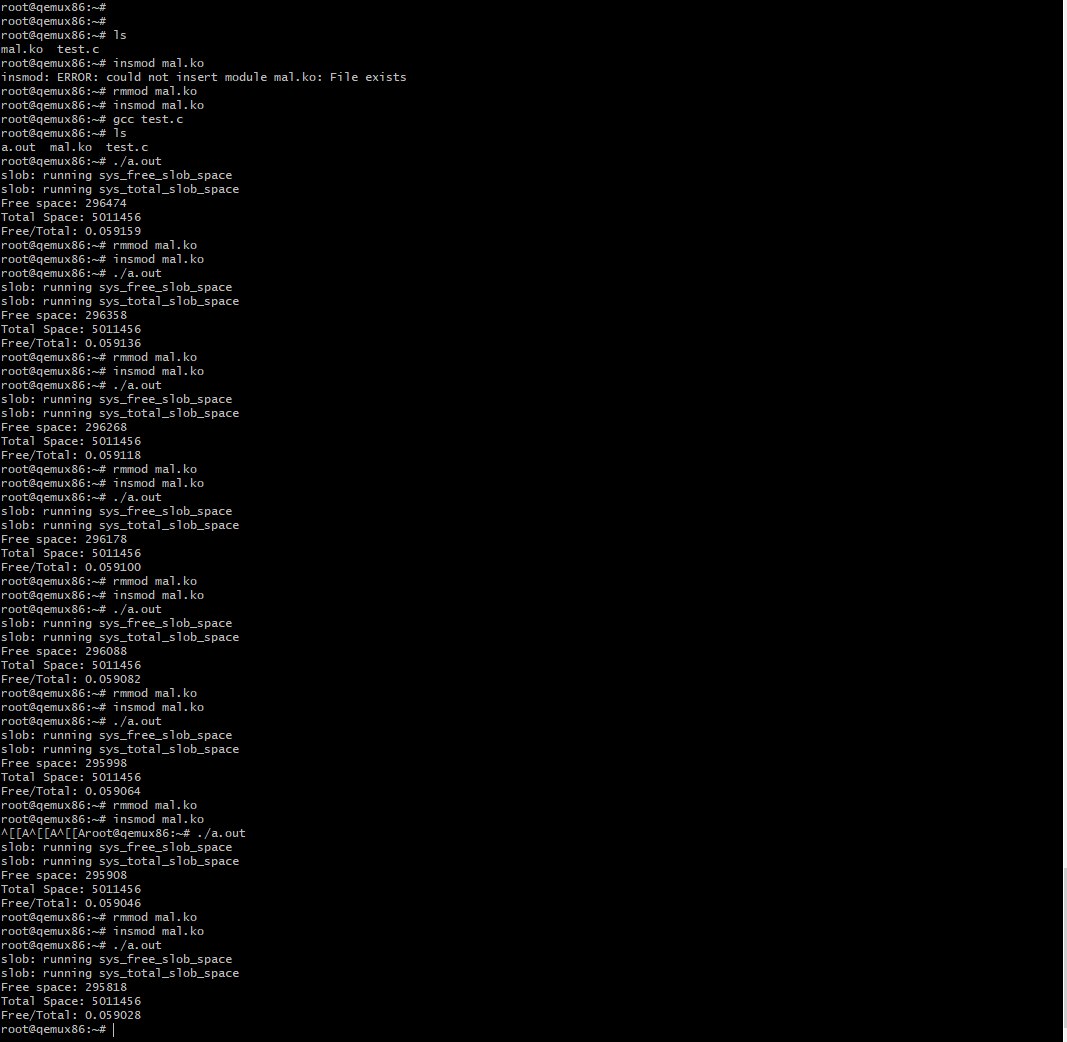
\includegraphics[width=\linewidth]{Best_fit.PNG}

First fit:\\
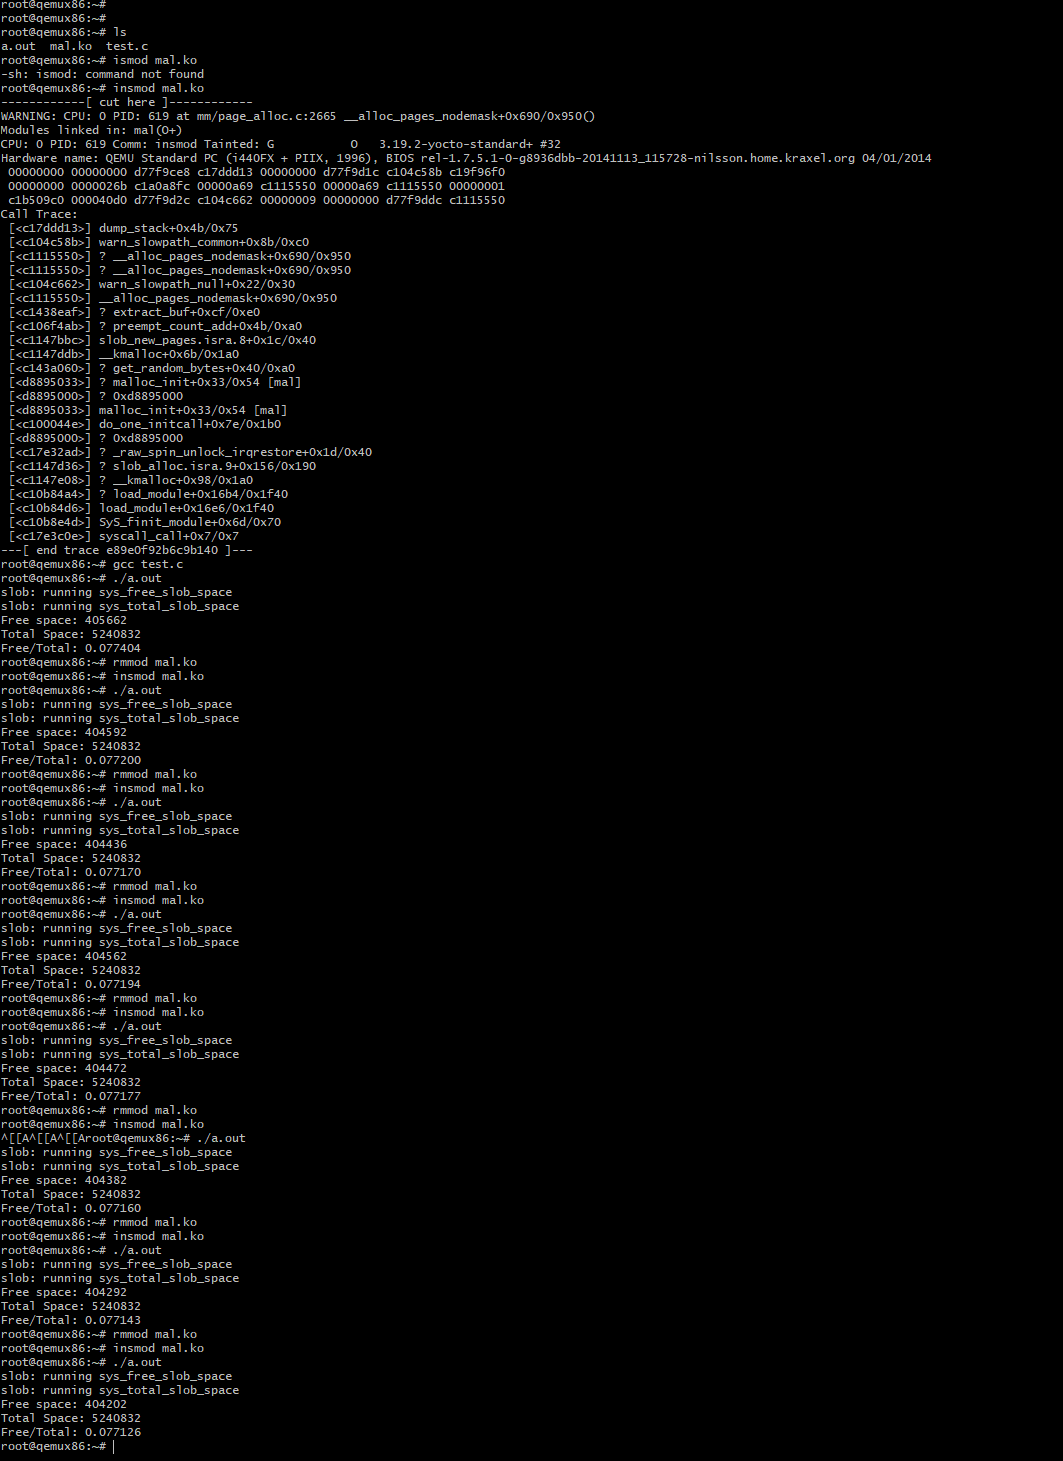
\includegraphics[width=\linewidth]{First_fit.PNG}
    \subsection{What did you learn?}
    We learned that the "best" fit algorithm, really was not the best fit for memory management. It contained too much overhead in memory and cost to be considered better than the first fit algorithm.\\

\newpage
\begin{landscape}

\section{Version Control log}
    \begin{center}
        \begin{tabular}{||c c c ||}
            \hline
            Author & Date & Message\\
            \hline \hline
            Thomas Noelcke noelcket@oregonstate.edu & 5/28/2018 & Started working on Algorithms\\
            \hline
            Thomas Noelcke anderrob@oregonstate.edu & 6/1/2018 & Worked on getting Algorithms to compile\\
            \hline
            Thomas Noelcke anderrob@oregonstate.edu & 6/5/2018 16:00 & Added System Calls\\
            \hline
            Hayden Anderson anderrob@oregonstate.edu & 6/5/2018 17:00 & worked on getting testing code up and running.\\
            \hline
            Hayden Anderson anderrob@oregonstate.edu & 6/6/2018 & got testing up and running.\\
            \hline
            Thomas Noelcke noelkcet@oregonstate.edu & 6/7/2018 & Finished up testing.\\
            \hline
        \end{tabular}
    \end{center}

\section{Work Log}
    	\begin{center}
			\begin{tabular}{||c c c c ||}
			\hline
			Name & Task & Date & Total Time\\[0.5ex]
			\hline \hline
			Thomas, Hayden and James & Researching Algorithms & 5/28 & 1 hour\\
			\hline
			Hayden & wrote out a design based off of previous research for the algorithms & 6/1 & 1.5 hours\\
			\hline
			Thomas & worked on getting algorithms we wrote earlier to compile & 6/3 & 2 hours\\
			\hline
			Thomas & Reworked the solution and added system calls & 6/5 & 4 hours\\
			\hline
			Hayden and James & worked on getting the testing script setup and how we were going to carry it out & 6/5 & 3 hours\\
			\hline
			Hayden & finished answering questions for hw and added some documentation & 6/6 & 1 hour\\
			\hline
			Hayden & got testing scripts to compile started to test them & 6/6 & 1 hour\\
			\hline
            Thomas, James & Finished testing and  worked on report & 6/7 & 1.5 hours\\
            \hline
            Thomas & Checked Commands and finished Git log & 6/7 & 1.5 hours\\
            \hline
			\end{tabular}
		\end{center}
\end{landscape}
\newpage


\end{document}
